\section{Tiefensuche}
\label{sect:tiefensuche}


\begin{bem} 
Die Eingabe für die hier diskutierte Tiefensuche ist ein Digraph $D=(V,A)$.
Ist der Graph ungerichtet, so ist die Vorgehensweise vollkommen analog und daher diskutieren wir hier (fast ausschließlich) die gerichtete Variante.
Der Digraph $D$ ist durch seine Adjazenzliste $N$ gegeben, das heißt, für jeden Knoten $u \in V$ ist $N[u]$ eine Liste aller $v \in V$ mit $(u,v) \in A$.
Die Darstellung von $D$ als Adjazenzliste eine Durchmusterung mit der optimalen Laufzeit $\Theta(|V|+|A|)$ erlaubt.
\end{bem}


\begin{bem} 
	Die Tiefensuche ist ein ``reiselustiger'' Algorithmus zur Durchmusterung von Graphen. Wenn wir Knoten als Orte auffassen und $N[u]$ als die Umgebung des Ortes $u$, so können wir das Grundgerüst der Tiefensuche so beschreiben. Man will alle noch nicht gesehenen Orte erkunden, die man von einem gegebenen Ort $u$ aus erreichen kann. Man kann dazu das folgende Vorgehen benutzen: 
	\begin{itemize} 
			\item Man sucht die Umgebung von $u$ durch. 
			\item Sobald man einen  noch nicht besuchten Ort $v$ sieht, erkundet man alle noch nicht gesehene Orte, die man von $v$ aus erreichen kann. 
	\end{itemize} 
	Der Grundgedanke  der Tiefensuche rekursiv: man erkundet neue Orte von $u$ aus, indem man die Orte erkunden, die man aus noch nicht gesehenen Nachbarschaft von $u$ erreichen kann. Die ``Reiselust'' dieser Durchmusterung besteht darin, dass man sich die Erkundung der Orte \emph{sofort} einen neuen Ort versetzt, wenn ein solcher Ort gefunden wird.  
	
	
	Bei rekursiven Algorithmen soll man sich bei der Umsetzung in der Regel als Erstes darum kümmern, dass der Algorithmus terminiert. Daher soll man bei der Durchmusterung die Orte, an die man kommt, gleich als ``gesehen'' markieren.  Stellen Sie sich einfach vor, dass Sie ein Stück Kreide nehmen und da, wo Sie angekommen sind, gleich schreiben ``hier war ich schon''. Sollten Sie bei Ihrer Wanderung durch den Graphen noch ein mal an diesen Ort kommen,  so werden Sie merken, dass Sie an diesem Ort bereits gewesen sind. Auf diese Weise werden Sie nicht endlos im Kreis herumlaufen, wenn etwa Ihr Graph ein Kreis ist oder einen Kreis enthält. 
	
	Die Umsetzung der oben beschriebenen Strategie basiert auf Farbattributen der Knoten, die man im Laufe der Durchmusterung sukzessiv zuerst als weiß ($=$ noch nicht gesehen), dann als  grau ($=$ gesehen aber noch nicht abgearbeitet) und schließlich als  schwarz ($=$ abgearbeitet) setzt. 
\end{bem}

\begin{defn}
	Wenn die Tiefensuche entlang einer Kante verläuft, die in einen weißen Knoten endet, dann sagen wir, dass der entsprechende Knoten \textbf{entdeckt} wird.

Hier eine Zusammenfassung der Bedeutung der Farben der Knoten.  
\begin{itemize}
	\item[] {\bfseries weiß:} Der Knoten wurde noch nicht entdeckt. 
	\item[] {\bfseries grau:} Der Knoten wurde entdeckt und die Tiefensuche für den Knoten läuft gerade.
	\item[] {\bfseries schwarz:} Der Knoten wurde entdeckt und die Tiefensuche für den Knoten ist bereits beendet.
\end{itemize}

Wird ein Knoten schwarz gefärbt, so sagen wir auch das er \textbf{abgearbeitet} wurde.

Durch die Tiefensuche können verschiedene Aufgaben erledigt werden. Nicht alle diese Aufgaben benötigen alle drei Farbattributen der Knoten. Bei manchen Aufgaben reicht auch die Unterscheidung zwischen ``entdeckt'' (weiß) und ``nicht entdeckt'' (grau oder schwarz) aus. 
\end{defn}

\begin{bem}
	Auf diese Weise können wir die Tiefensuche initialisiert: 
	\begin{algorithm} 
		\caption{$\cc{Tiefensuche-Initialisieren}(D)$}
	\begin{algorithmic}[1]
		\FOR{$u \in V$}
		\STATE $\cc{Farbe}[u]=\cc{weiß}$
		\STATE $\pi[u]=\cc{nil}$
		\ENDFOR
		\end{algorithmic}
	\end{algorithm} 
\end{bem}  


\begin{bem} Sobald die Initialisierung erfolgt ist, können wir die Tiefensuche von einem gegebenen Knoten ausführen. Hier die rekursive Umsetzung: 
	\begin{algorithm}[H]
		\caption{$\cc{Tiefensuche}(u)$}
		\begin{algorithmic}[1]
			\STATE $\cc{Farbe}[u]:=\cc{grau}$ \ \COMMENT{$u$ als entdeckt notiert} 
			\FOR{$v \in N[u]$}
			\STATE  \COMMENT{Die Kante $(u,v)$ wird sondiert}
			\IF{$\cc{Farbe}[v]=\cc{weiß}$}
			\STATE $\pi[v]:=u$   \ \COMMENT{Knoten $v$ wurde entdeckt} 
			\STATE $\cc{Tiefensuche}(v)$
			\ENDIF
			\ENDFOR
			\STATE $\cc{Farbe}[u]:=\cc{schwarz}$ 
		\end{algorithmic}
	\end{algorithm}
\end{bem}

\begin{bem} 
	Die Prozedur Tiefensuche können wir in den folgenden Rahmen einbauen. 
	\begin{algorithm}[H]
		\caption{$\cc{Vollständige-Tiefensuche}(D)$}
		\begin{algorithmic}[1]
			\STATE $\cc{Tiefensuche-Initialisieiren}(D)$ 
			\FOR{$u \in V$}\label{line:tiefensuche-hauptschleife-start}
			\IF{$\cc{Farbe}[u]=\cc{weiß}$}
			\STATE $\cc{Tiefensuche}(u)$
			\ENDIF 
			\ENDFOR\label{line:tiefensuche-hauptschleife-ende}
		\end{algorithmic}
	\end{algorithm}
	Durch diese Prozedur entdecken wir jeden jeden Knoten genau ein mal und sondieren dabei jede Kante von $D=(V,A)$. 
\end{bem}




\begin{bem}[Variante mit Zeitstempeln] 
 Jeder Knoten $v \in V$ kann während der Tiefensuche mit zwei \emph{Zeitstempeln} versehen werden: Der erste Zeitstempel $\cc{Grau}[v]$ zeichnet auf, wann der Knoten grau gefärbt wird, das heißt, wann er das erste Mal entdeckt wird.
Der zweite Zeitstempel $\cc{Schwarz}[v]$ hingegen, speichert den Zeitpunkt der Schwarzfärbung von~$v$, das heißt, den Moment in dem der Knoten abgearbeitet ist.

Im Algorithmus werden beide Zeitstempel ganze Zahlen zwischen $1$ und $2 |V|$ sein, da es für jeden Knoten $v \in V$ genau einen Zeitpunkt der Entdeckung (Graufärbung) und einen Zeitpunkt der Abarbeitung (Schwarzfärbung) gibt.

Für jedes $v \in V$ gilt $\cc{Grau}[v] < \cc{Schwarz}[v]$.
Weiterhin ist $v$ vor dem Zeitpunkt $\cc{Grau}[v]$ weiß, während der Zeitpunkte $\cc{Grau}[v],\ldots,\cc{Schwarz}[v]-1$ grau, und ab dem Zeitpunkt $\cc{Schwarz}[v]$ schwarz.

Für die Variante mit den Zeitstempeln sollen die Initialisierung und die Tiefensuche geringfügig ergänzt werden. 

Die Initialisierung: 

	\begin{algorithm} 
	\caption{$\cc{Tiefensuche-Initialisieren}(D)$}
	\begin{algorithmic}[1]
		\FOR{$u \in V$}
		\STATE $\cc{Farbe}[u]=\cc{weiß}$
		\STATE $\pi[u]=\cc{nil}$
		\ENDFOR
		\STATE {\color{red} $t:=0$ \quad \COMMENT{Initialisierung der Zeit-Variablen} }
	\end{algorithmic}
\end{algorithm} 

Die Tiefensuche: 

\begin{algorithm}[H]
	\caption{$\cc{Tiefensuche}(u)$}
	\begin{algorithmic}[1]
		\STATE {\color{red} $t := t + 1$ $\quad$ \COMMENT{Die Uhr tickt vor jeder Färbung} }
		\STATE { \color{red} $\cc{Grau}[u] := t$ $\quad$ \COMMENT{Der Knoten $u$ wurde gerade entdeckt} }
		\STATE $\cc{Farbe}[u]:=\cc{grau}$
		\FOR{$v \in N[u]$}
		\IF{$\cc{Farbe}[v]=\cc{weiß}$}
		 \STATE $\pi[v]:=u$  
		\STATE $\cc{Tiefensuche}(v)$
		\ENDIF
		\ENDFOR
		\STATE {\color{red} $t := t + 1$ $\quad$ \COMMENT{Die Uhr tickt vor jeder Färbung} }
		\STATE\label{line:schwarzfaerbung-in-tiefensuche} {\color{red} $\cc{Schwarz}[u] := t$ $\quad$ \COMMENT{Der Knoten $u$ wurde gerade abgearbeitet}}
		\STATE $\cc{Farbe}[u]:=\cc{schwarz}$
	\end{algorithmic}
\end{algorithm}
\end{bem}

\begin{bsp}
\label{bsp:tiefensuche}
Wir illustrieren die Tiefensuche am Digraphen

\hfill
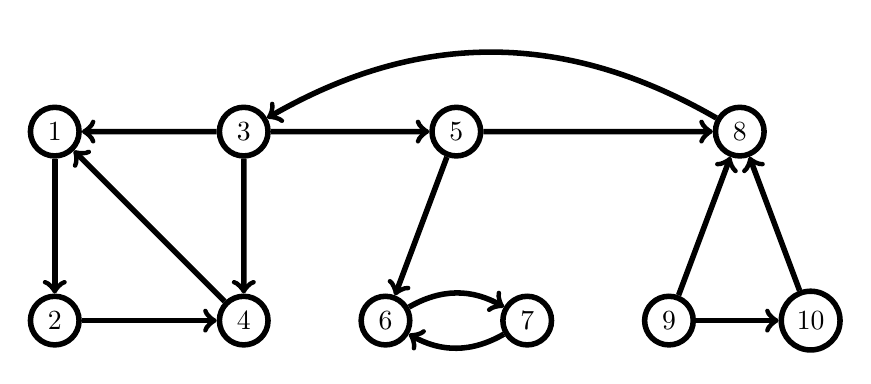
\begin{tikzpicture}[line width=2,scale=1.2]
 \node[circle,draw=black] (1) at (0,2) {$1$};
 \node[circle,draw=black] (2) at (0,0) {$2$};
 \node[circle,draw=black] (3) at (2,2) {$3$};
 \node[circle,draw=black] (4) at (2,0) {$4$};
 \node[circle,draw=black] (5) at (4.25,2) {$5$};
 \node[circle,draw=black] (6) at (3.5,0) {$6$};
 \node[circle,draw=black] (7) at (5,0) {$7$};
 \node[circle,draw=black] (8) at (7.25,2) {$8$};
 \node[circle,draw=black] (9) at (6.5,0) {$9$};
 \node[circle,draw=black] (10) at (8,0) {$10$};
		
 \draw[->] (1) edge (2);
 \draw[->] (2) edge (4);
 \draw[->] (3) edge (1) (3) edge (4) (3) edge (5);
 \draw[->] (4) edge (1);
 \draw[->] (5) edge (6) (5) edge (8); 
 \draw[->] (6) to[bend left] (7);
 \draw[->] (7) to[bend left] (6);
 \draw[->] (8) to[bend right] (3);
 \draw[->] (9) edge (8) (9) edge (10);
 \draw[->] (10) edge (8); 
\end{tikzpicture}
\hfill\,

Wir wählen als Startknoten den Knoten~$3$ und treffen ansonsten jede Wahl aufsteigend in der Reihenfolge der Knotenindizes.
Die ersten sechs Zeitschritte sind durch die folgende Sequenz von gefärbten Digraphen gegeben, wobei die Knotenfarbe dem aktuellen Farbattribut entspricht und die bereits sondierten Kanten rot markiert sind:

\condclearpage 

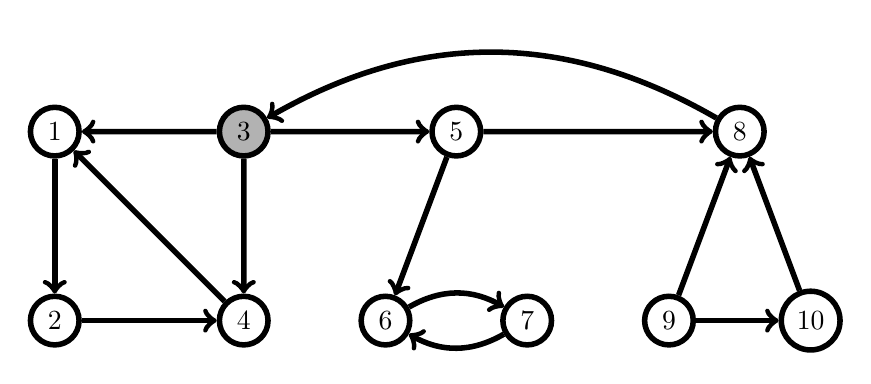
\begin{tikzpicture}[line width=2,scale=1.2]
 \tikzset{gnode/.style ={fill=black!30!,circle,draw}}
 \tikzset{snode/.style ={white,fill=black,circle,draw}}

 \node[circle,draw=black] (1) at (0,2) {$1$};
 \node[circle,draw=black] (2) at (0,0) {$2$};
 \node[gnode] (3) at (2,2) {$3$};
 \node[circle,draw=black] (4) at (2,0) {$4$};
 \node[circle,draw=black] (5) at (4.25,2) {$5$};
 \node[circle,draw=black] (6) at (3.5,0) {$6$};
 \node[circle,draw=black] (7) at (5,0) {$7$};
 \node[circle,draw=black] (8) at (7.25,2) {$8$};
 \node[circle,draw=black] (9) at (6.5,0) {$9$};
 \node[circle,draw=black] (10) at (8,0) {$10$};
		
 \draw[->] (1) edge (2);
 \draw[->] (2) edge (4);
 \draw[->] (3) edge (1) (3) edge (4) (3) edge (5);
 \draw[->] (4) edge (1);
 \draw[->] (5) edge (6) (5) edge (8); 
 \draw[->] (6) to[bend left] (7);
 \draw[->] (7) to[bend left] (6);
 \draw[->] (8) to[bend right] (3);
 \draw[->] (9) edge (8) (9) edge (10);
 \draw[->] (10) edge (8); 
\end{tikzpicture}
\\ $TS(3)$ 

\condclearpage 

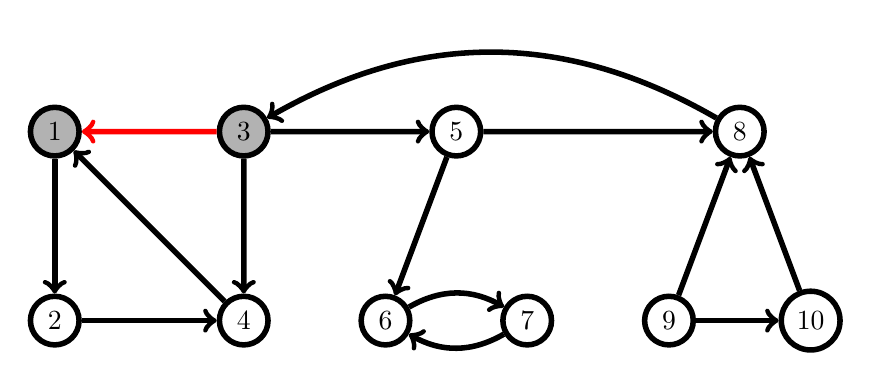
\begin{tikzpicture}[line width=2,scale=1.2]
 \tikzset{gnode/.style ={fill=black!30!,circle,draw}}
 \tikzset{snode/.style ={white,fill=black,circle,draw}}

 \node[gnode] (1) at (0,2) {$1$};
 \node[circle,draw=black] (2) at (0,0) {$2$};
 \node[gnode] (3) at (2,2) {$3$};
 \node[circle,draw=black] (4) at (2,0) {$4$};
 \node[circle,draw=black] (5) at (4.25,2) {$5$};
 \node[circle,draw=black] (6) at (3.5,0) {$6$};
 \node[circle,draw=black] (7) at (5,0) {$7$};
 \node[circle,draw=black] (8) at (7.25,2) {$8$};
 \node[circle,draw=black] (9) at (6.5,0) {$9$};
 \node[circle,draw=black] (10) at (8,0) {$10$};
		
 \draw[->] (1) edge (2);
 \draw[->] (2) edge (4);
 \draw[->,red] (3) edge (1);
 \draw[->] (3) edge (4) (3) edge (5);
 \draw[->] (4) edge (1);
 \draw[->] (5) edge (6) (5) edge (8); 
 \draw[->] (6) to[bend left] (7);
 \draw[->] (7) to[bend left] (6);
 \draw[->] (8) to[bend right] (3);
 \draw[->] (9) edge (8) (9) edge (10);
 \draw[->] (10) edge (8); 
\end{tikzpicture}
\\ $TS(3) \to TS(1)$ 

\condclearpage 
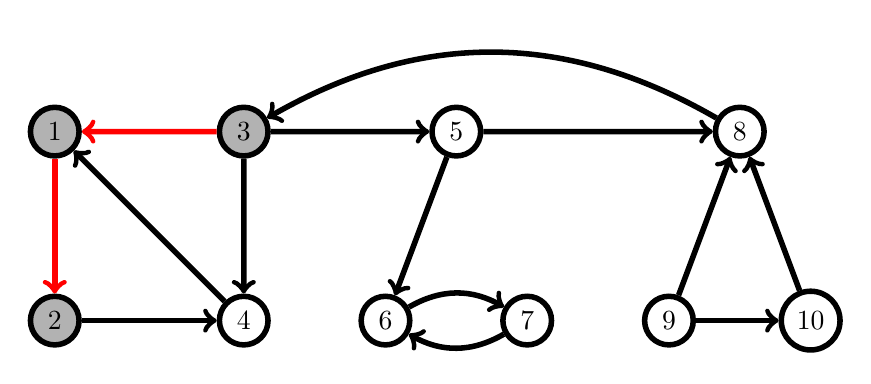
\begin{tikzpicture}[line width=2,scale=1.2]
 \tikzset{gnode/.style ={fill=black!30!,circle,draw}}
 \tikzset{snode/.style ={white,fill=black,circle,draw}}

 \node[gnode] (1) at (0,2) {$1$};
 \node[gnode] (2) at (0,0) {$2$};
 \node[gnode] (3) at (2,2) {$3$};
 \node[circle,draw=black] (4) at (2,0) {$4$};
 \node[circle,draw=black] (5) at (4.25,2) {$5$};
 \node[circle,draw=black] (6) at (3.5,0) {$6$};
 \node[circle,draw=black] (7) at (5,0) {$7$};
 \node[circle,draw=black] (8) at (7.25,2) {$8$};
 \node[circle,draw=black] (9) at (6.5,0) {$9$};
 \node[circle,draw=black] (10) at (8,0) {$10$};
		
 \draw[->,red] (1) edge (2);
 \draw[->] (2) edge (4);
 \draw[->,red] (3) edge (1);
 \draw[->] (3) edge (4) (3) edge (5);
 \draw[->] (4) edge (1);
 \draw[->] (5) edge (6) (5) edge (8); 
 \draw[->] (6) to[bend left] (7);
 \draw[->] (7) to[bend left] (6);
 \draw[->] (8) to[bend right] (3);
 \draw[->] (9) edge (8) (9) edge (10);
 \draw[->] (10) edge (8); 
\end{tikzpicture}
\\ $TS(3)\to TS(1) \to TS(2)$  

\condclearpage 
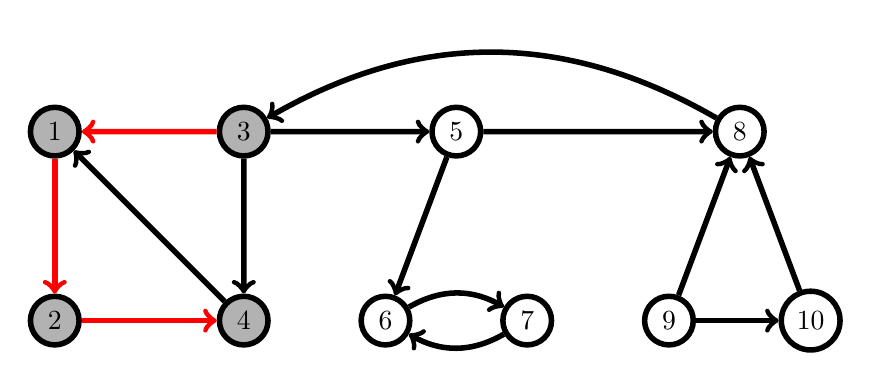
\begin{tikzpicture}[line width=2,scale=1.2]
 \tikzset{gnode/.style ={fill=black!30!,circle,draw}}
 \tikzset{snode/.style ={white,fill=black,circle,draw}}

 \node[gnode] (1) at (0,2) {$1$};
 \node[gnode] (2) at (0,0) {$2$};
 \node[gnode] (3) at (2,2) {$3$};
 \node[gnode] (4) at (2,0) {$4$};
 \node[circle,draw=black] (5) at (4.25,2) {$5$};
 \node[circle,draw=black] (6) at (3.5,0) {$6$};
 \node[circle,draw=black] (7) at (5,0) {$7$};
 \node[circle,draw=black] (8) at (7.25,2) {$8$};
 \node[circle,draw=black] (9) at (6.5,0) {$9$};
 \node[circle,draw=black] (10) at (8,0) {$10$};
		
 \draw[->,red] (1) edge (2);
 \draw[->,red] (2) edge (4);
 \draw[->,red] (3) edge (1);
 \draw[->] (3) edge (4) (3) edge (5);
 \draw[->] (4) edge (1);
 \draw[->] (5) edge (6) (5) edge (8); 
 \draw[->] (6) to[bend left] (7);
 \draw[->] (7) to[bend left] (6);
 \draw[->] (8) to[bend right] (3);
 \draw[->] (9) edge (8) (9) edge (10);
 \draw[->] (10) edge (8); 
\end{tikzpicture}
\\ $TS(3)\to TS(1) \to TS(2) \to TS(4)$ 

\condclearpage
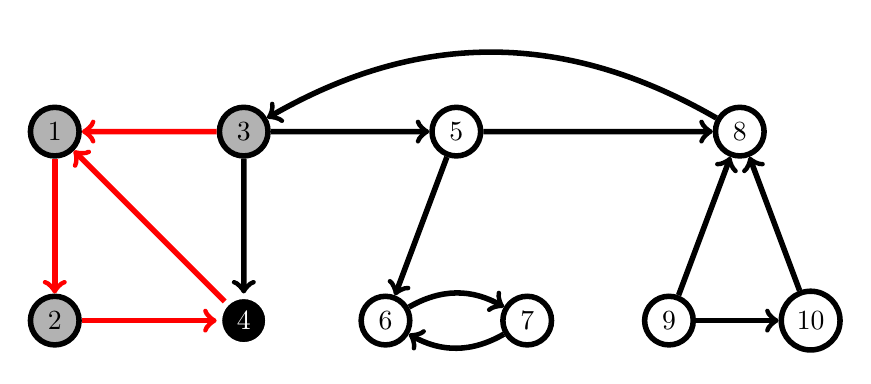
\begin{tikzpicture}[line width=2,scale=1.2]
 \tikzset{gnode/.style ={fill=black!30!,circle,draw}}
\tikzset{snode/.style ={white,fill=black,circle,draw}}

 \node[gnode] (1) at (0,2) {$1$};
 \node[gnode] (2) at (0,0) {$2$};
 \node[gnode] (3) at (2,2) {$3$};
 \node[snode] (4) at (2,0) {$4$};
 \node[circle,draw=black] (5) at (4.25,2) {$5$};
 \node[circle,draw=black] (6) at (3.5,0) {$6$};
 \node[circle,draw=black] (7) at (5,0) {$7$};
 \node[circle,draw=black] (8) at (7.25,2) {$8$};
 \node[circle,draw=black] (9) at (6.5,0) {$9$};
 \node[circle,draw=black] (10) at (8,0) {$10$};
		
 \draw[->,red] (1) edge (2);
 \draw[->,red] (2) edge (4);
 \draw[->,red] (3) edge (1);
 \draw[->] (3) edge (4) (3) edge (5);
 \draw[->,red] (4) edge (1);
 \draw[->] (5) edge (6) (5) edge (8); 
 \draw[->] (6) to[bend left] (7);
 \draw[->] (7) to[bend left] (6);
 \draw[->] (8) to[bend right] (3);
 \draw[->] (9) edge (8) (9) edge (10);
 \draw[->] (10) edge (8); 
\end{tikzpicture}
\\ $TS(3)\to TS(1) \to TS(2)$

\condclearpage 
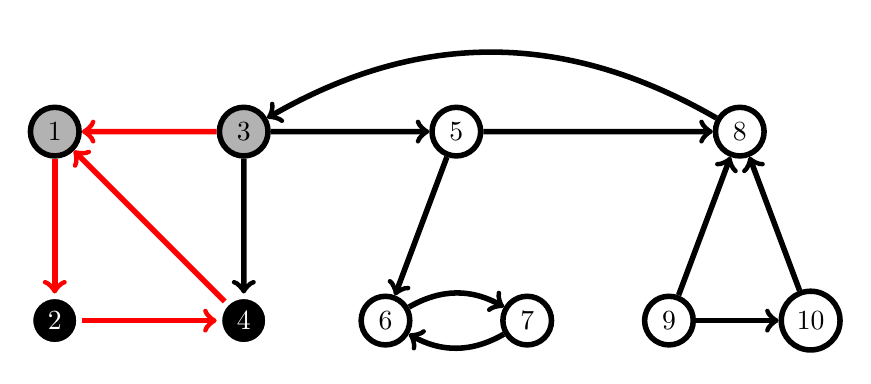
\begin{tikzpicture}[line width=2,scale=1.2]
 \tikzset{gnode/.style ={fill=black!30!,circle,draw}}
 \tikzset{snode/.style ={white,fill=black,circle,draw}}

 \node[gnode] (1) at (0,2) {$1$};
 \node[snode] (2) at (0,0) {$2$};
 \node[gnode] (3) at (2,2) {$3$};
 \node[snode] (4) at (2,0) {$4$};
 \node[circle,draw=black] (5) at (4.25,2) {$5$};
 \node[circle,draw=black] (6) at (3.5,0) {$6$};
 \node[circle,draw=black] (7) at (5,0) {$7$};
 \node[circle,draw=black] (8) at (7.25,2) {$8$};
 \node[circle,draw=black] (9) at (6.5,0) {$9$};
 \node[circle,draw=black] (10) at (8,0) {$10$};
		
 \draw[->,red] (1) edge (2);
 \draw[->,red] (2) edge (4);
 \draw[->,red] (3) edge (1);
 \draw[->] (3) edge (4) (3) edge (5);
 \draw[->,red] (4) edge (1);
 \draw[->] (5) edge (6) (5) edge (8); 
 \draw[->] (6) to[bend left] (7);
 \draw[->] (7) to[bend left] (6);
 \draw[->] (8) to[bend right] (3);
 \draw[->] (9) edge (8) (9) edge (10);
 \draw[->] (10) edge (8); 
\end{tikzpicture}
\\ $TS(3)\to TS(1)$

Wir steigen zum Zeitpunkt $\cc{Schwarz}[8]=14$ mit der Illustration wieder ein:

\condclearpage 
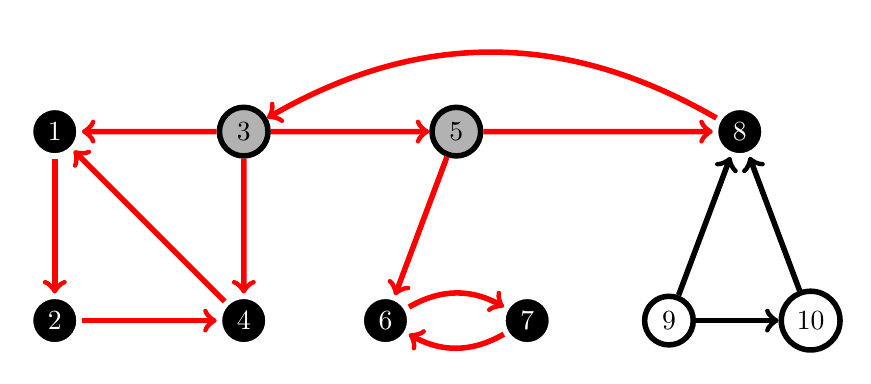
\begin{tikzpicture}[line width=2,scale=1.2]
 \tikzset{gnode/.style ={fill=black!30!,circle,draw}}
 \tikzset{snode/.style ={white,fill=black,circle,draw}}

 \node[snode] (1) at (0,2) {$1$};
 \node[snode] (2) at (0,0) {$2$};
 \node[gnode] (3) at (2,2) {$3$};
 \node[snode] (4) at (2,0) {$4$};
 \node[gnode] (5) at (4.25,2) {$5$};
 \node[snode] (6) at (3.5,0) {$6$};
 \node[snode] (7) at (5,0) {$7$};
 \node[snode] (8) at (7.25,2) {$8$};
 \node[circle,draw=black] (9) at (6.5,0) {$9$};
 \node[circle,draw=black] (10) at (8,0) {$10$};
		
 \draw[->,red] (1) edge (2);
 \draw[->,red] (2) edge (4);
 \draw[->,red] (3) edge (1);
 \draw[->,red] (3) edge (4) (3) edge (5);
 \draw[->,red] (4) edge (1);
 \draw[->,red] (5) edge (6) (5) edge (8); 
 \draw[->,red] (6) to[bend left] (7);
 \draw[->,red] (7) to[bend left] (6);
 \draw[->,red] (8) to[bend right] (3);
 \draw[->] (9) edge (8) (9) edge (10);
 \draw[->] (10) edge (8); 
\end{tikzpicture}
\\ $TS(3)\to TS(5)$

\condclearpage 
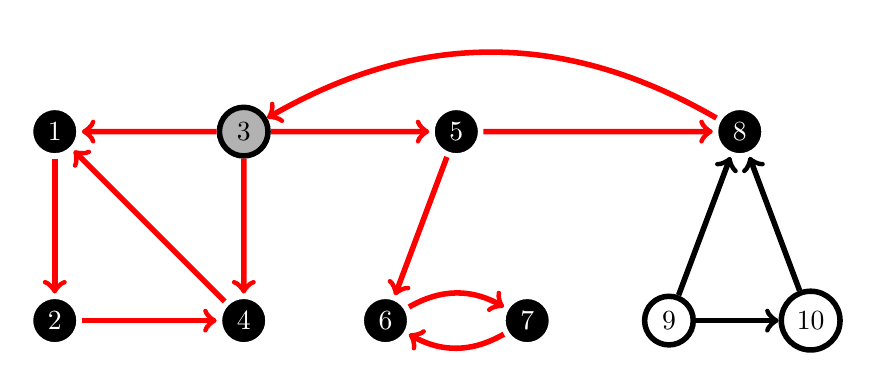
\begin{tikzpicture}[line width=2,scale=1.2]
 \tikzset{gnode/.style ={fill=black!30!,circle,draw}}
 \tikzset{snode/.style ={white,fill=black,circle,draw}}

 \node[snode] (1) at (0,2) {$1$};
 \node[snode] (2) at (0,0) {$2$};
 \node[gnode] (3) at (2,2) {$3$};
 \node[snode] (4) at (2,0) {$4$};
 \node[snode] (5) at (4.25,2) {$5$};
 \node[snode] (6) at (3.5,0) {$6$};
 \node[snode] (7) at (5,0) {$7$};
 \node[snode] (8) at (7.25,2) {$8$};
 \node[circle,draw=black] (9) at (6.5,0) {$9$};
 \node[circle,draw=black] (10) at (8,0) {$10$};
		
 \draw[->,red] (1) edge (2);
 \draw[->,red] (2) edge (4);
 \draw[->,red] (3) edge (1);
 \draw[->,red] (3) edge (4) (3) edge (5);
 \draw[->,red] (4) edge (1);
 \draw[->,red] (5) edge (6) (5) edge (8); 
 \draw[->,red] (6) to[bend left] (7);
 \draw[->,red] (7) to[bend left] (6);
 \draw[->,red] (8) to[bend right] (3);
 \draw[->] (9) edge (8) (9) edge (10);
 \draw[->] (10) edge (8); 
\end{tikzpicture}
\hfill\,

\condclearpage 
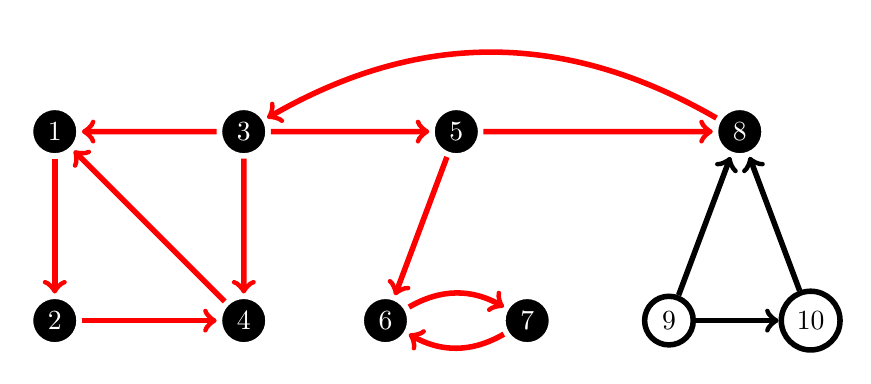
\begin{tikzpicture}[line width=2,scale=1.2]
 \tikzset{gnode/.style ={fill=black!30!,circle,draw}}
 \tikzset{snode/.style ={white,fill=black,circle,draw}}

 \node[snode] (1) at (0,2) {$1$};
 \node[snode] (2) at (0,0) {$2$};
 \node[snode] (3) at (2,2) {$3$};
 \node[snode] (4) at (2,0) {$4$};
 \node[snode] (5) at (4.25,2) {$5$};
 \node[snode] (6) at (3.5,0) {$6$};
 \node[snode] (7) at (5,0) {$7$};
 \node[snode] (8) at (7.25,2) {$8$};
 \node[circle,draw=black] (9) at (6.5,0) {$9$};
 \node[circle,draw=black] (10) at (8,0) {$10$};
		
 \draw[->,red] (1) edge (2);
 \draw[->,red] (2) edge (4);
 \draw[->,red] (3) edge (1);
 \draw[->,red] (3) edge (4) (3) edge (5);
 \draw[->,red] (4) edge (1);
 \draw[->,red] (5) edge (6) (5) edge (8); 
 \draw[->,red] (6) to[bend left] (7);
 \draw[->,red] (7) to[bend left] (6);
 \draw[->,red] (8) to[bend right] (3);
 \draw[->] (9) edge (8) (9) edge (10);
 \draw[->] (10) edge (8); 
\end{tikzpicture}
\hfill\,

Nun muss ein neuer Knoten gewählt werden (Knoten $9$) um die Tiefensuche für den ganzen Digraphen zu beenden:

\condclearpage 
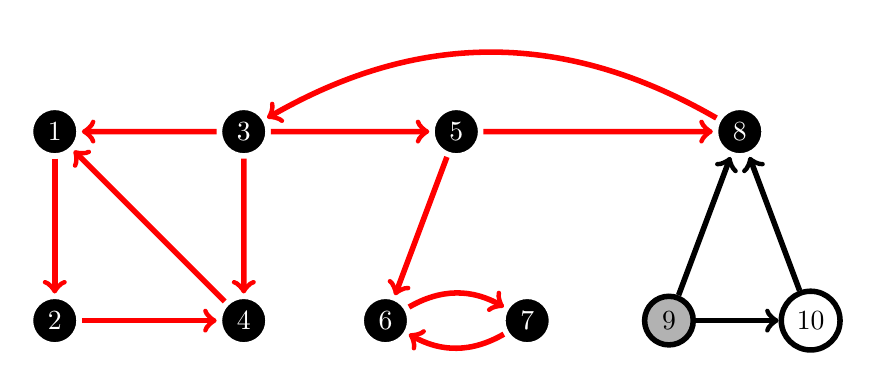
\begin{tikzpicture}[line width=2,scale=1.2]
 \tikzset{gnode/.style ={fill=black!30!,circle,draw}}
 \tikzset{snode/.style ={white,fill=black,circle,draw}}

 \node[snode] (1) at (0,2) {$1$};
 \node[snode] (2) at (0,0) {$2$};
 \node[snode] (3) at (2,2) {$3$};
 \node[snode] (4) at (2,0) {$4$};
 \node[snode] (5) at (4.25,2) {$5$};
 \node[snode] (6) at (3.5,0) {$6$};
 \node[snode] (7) at (5,0) {$7$};
 \node[snode] (8) at (7.25,2) {$8$};
 \node[gnode] (9) at (6.5,0) {$9$};
 \node[circle,draw=black] (10) at (8,0) {$10$};
		
 \draw[->,red] (1) edge (2);
 \draw[->,red] (2) edge (4);
 \draw[->,red] (3) edge (1);
 \draw[->,red] (3) edge (4) (3) edge (5);
 \draw[->,red] (4) edge (1);
 \draw[->,red] (5) edge (6) (5) edge (8); 
 \draw[->,red] (6) to[bend left] (7);
 \draw[->,red] (7) to[bend left] (6);
 \draw[->,red] (8) to[bend right] (3);
 \draw[->] (9) edge (8) (9) edge (10);
 \draw[->] (10) edge (8); 
\end{tikzpicture}
\hfill\,

\condclearpage 
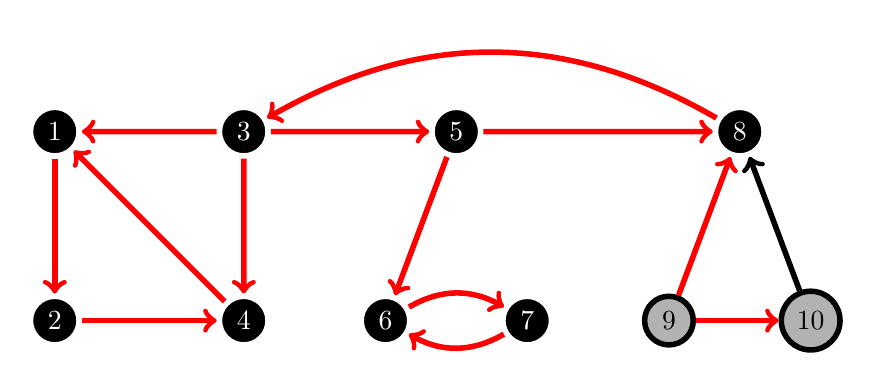
\begin{tikzpicture}[line width=2,scale=1.2]
 \tikzset{gnode/.style ={fill=black!30!,circle,draw}}
 \tikzset{snode/.style ={white,fill=black,circle,draw}}

 \node[snode] (1) at (0,2) {$1$};
 \node[snode] (2) at (0,0) {$2$};
 \node[snode] (3) at (2,2) {$3$};
 \node[snode] (4) at (2,0) {$4$};
 \node[snode] (5) at (4.25,2) {$5$};
 \node[snode] (6) at (3.5,0) {$6$};
 \node[snode] (7) at (5,0) {$7$};
 \node[snode] (8) at (7.25,2) {$8$};
 \node[gnode] (9) at (6.5,0) {$9$};
 \node[gnode] (10) at (8,0) {$10$};
		
 \draw[->,red] (1) edge (2);
 \draw[->,red] (2) edge (4);
 \draw[->,red] (3) edge (1);
 \draw[->,red] (3) edge (4) (3) edge (5);
 \draw[->,red] (4) edge (1);
 \draw[->,red] (5) edge (6) (5) edge (8); 
 \draw[->,red] (6) to[bend left] (7);
 \draw[->,red] (7) to[bend left] (6);
 \draw[->,red] (8) to[bend right] (3);
 \draw[->,red] (9) edge (8) (9) edge (10);
 \draw[->] (10) edge (8); 
\end{tikzpicture}
\hfill\,

\condclearpage 
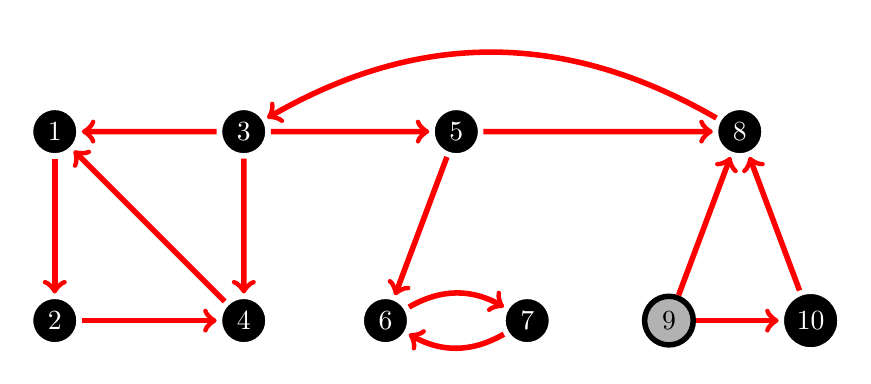
\begin{tikzpicture}[line width=2,scale=1.2]
 \tikzset{gnode/.style ={fill=black!30!,circle,draw}}
 \tikzset{snode/.style ={white,fill=black,circle,draw}}

 \node[snode] (1) at (0,2) {$1$};
 \node[snode] (2) at (0,0) {$2$};
 \node[snode] (3) at (2,2) {$3$};
 \node[snode] (4) at (2,0) {$4$};
 \node[snode] (5) at (4.25,2) {$5$};
 \node[snode] (6) at (3.5,0) {$6$};
 \node[snode] (7) at (5,0) {$7$};
 \node[snode] (8) at (7.25,2) {$8$};
 \node[gnode] (9) at (6.5,0) {$9$};
 \node[snode] (10) at (8,0) {$10$};
		
 \draw[->,red] (1) edge (2);
 \draw[->,red] (2) edge (4);
 \draw[->,red] (3) edge (1);
 \draw[->,red] (3) edge (4) (3) edge (5);
 \draw[->,red] (4) edge (1);
 \draw[->,red] (5) edge (6) (5) edge (8); 
 \draw[->,red] (6) to[bend left] (7);
 \draw[->,red] (7) to[bend left] (6);
 \draw[->,red] (8) to[bend right] (3);
 \draw[->,red] (9) edge (8) (9) edge (10);
 \draw[->,red] (10) edge (8); 
\end{tikzpicture}
\hfill\,

\condclearpage 
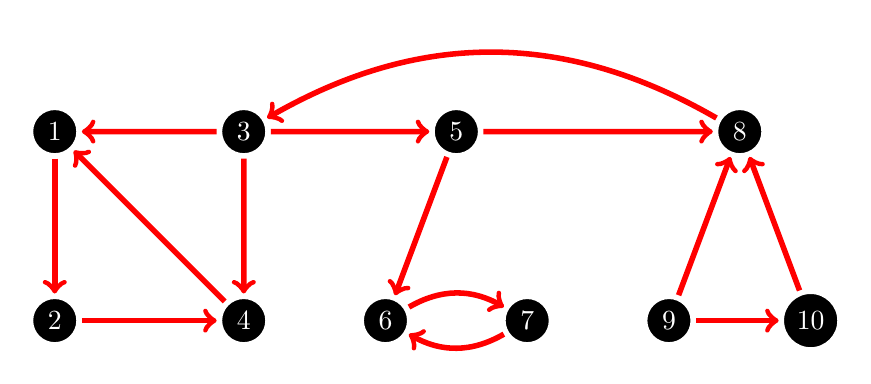
\begin{tikzpicture}[line width=2,scale=1.2]
 \tikzset{gnode/.style ={fill=black!30!,circle,draw}}
 \tikzset{snode/.style ={white,fill=black,circle,draw}}

 \node[snode] (1) at (0,2) {$1$};
 \node[snode] (2) at (0,0) {$2$};
 \node[snode] (3) at (2,2) {$3$};
 \node[snode] (4) at (2,0) {$4$};
 \node[snode] (5) at (4.25,2) {$5$};
 \node[snode] (6) at (3.5,0) {$6$};
 \node[snode] (7) at (5,0) {$7$};
 \node[snode] (8) at (7.25,2) {$8$};
 \node[snode] (9) at (6.5,0) {$9$};
 \node[snode] (10) at (8,0) {$10$};
		
 \draw[->,red] (1) edge (2);
 \draw[->,red] (2) edge (4);
 \draw[->,red] (3) edge (1);
 \draw[->,red] (3) edge (4) (3) edge (5);
 \draw[->,red] (4) edge (1);
 \draw[->,red] (5) edge (6) (5) edge (8); 
 \draw[->,red] (6) to[bend left] (7);
 \draw[->,red] (7) to[bend left] (6);
 \draw[->,red] (8) to[bend right] (3);
 \draw[->,red] (9) edge (8) (9) edge (10);
 \draw[->,red] (10) edge (8); 
\end{tikzpicture}
\hfill\,

Nun sind alle Knoten schwarz und die Tiefensuche ist beendet.
\end{bsp}

%Als Beispiel kann man die TS mit dem Startknoten $1$ im Fall von $N$:
%\[
%	\begin{array}{llll}
%	1: & 2, & 4 
%	\\ 2: & 3
%	\\ 3: & 
%	\\ 4: & 2, & 3, & 5
%	\\ 5: & 6
%	\\ 6: & 4
%	\\ 7: & 6
%	\end{array}
%\]
%betrachten. Wir protokollieren die Änderungen wann welche TSen aufgerufen und beendet werden und wie sich die Farben der Knoten ändern. *****

\begin{bem}
	Bevor wir die Anwendungen der Tiefensuche diskutieren, analysieren wir Ihre Laufzeit. 
\end{bem} 

\begin{thm}
\label{thm:laufzeit-tiefensuche}
Es sei ein Digraph $D=(V,A)$ durch eine Adjazenzliste gegeben. Dann hat die Laufzeit von $\cc{Tiefensuche}(s)$ die Ordnung $O(|V|+|A|)$ und die  Laufzeit von $\cc{Vollständige-Tiefensuche}(D)$ die Ordnung $\Theta(|V|+|A|)$.
\end{thm}

\begin{proof}
Der Aufwand setzt sich aus aus den folgenden Operationen zusammen, die man den Knoten und Kanten zuordnet: 

\begin{equation*}
	\cc{weiss} 
	\ \xrightarrow{\text{$TS(u)$ Start}} \ 
	\cc{grau}
	\ \xrightarrow{\text{Sondierung von $N[u]$}}
	\ \cc{schwarz} 
	\  \xrightarrow{\text{$TS(u)$ Ende}} \ 
\end{equation*} 

Hier wird $TS$ als Abkürzung für $\cc{Tiefensuche}$ benutzt. Für die Tiefensuche und vollständige Tiefensuche ist der Aufwand somit höchstens $O(|V|+|E|)$, denn der Aufwand pro Konten  $O(1)$, da kein Knoten $u$ wegen der Änderung der Farben mehr als ein mal sondiert werden kann. Genau so ist der Aufwand pro jede Kante $O(1)$, da eine Kante $(u,v)$ genau dann sondiert wird, wenn man $u$ entdeckt, der Knoten $u$ wird aber höchstens ein mal entdeckt. 

Es ist klar, dass der Aufwand bei der vollständigen Tiefensuche $\Omega(|V|+|A|)$, da die For-Schleife in der vollständige Tiefensuche dafür sorgt, dass jeder Knoten ein mal entdeckt wird. 
\end{proof}


%\begin{thm}
%	Sei $G=(V,E)$ Digraph mit $m \in \N$ Kanten und $n \in \N$ Knoten, der durch eine Adjazenzliste gegeben ist. Sei $s \in V$. Dan gilt für die Tiefensuche auf $G$ mit dem Startknoten $s$:
%	\begin{enumerate}[(a)]
%		\item Die Laufzeit des Verfahrens ist $O(m+n)$ (das heißt, höchstens $c(m+n)$ für eine Konstante $c>0$).
%		\item Die Menge aller Knoten von $G$, die von $s$ aus durch einen Pfad erreichbar sind ist genau die Menge der Knoten, die während der Ausführung entdeckt werden. 
%		\item Der Graph $G$ enthält genau dann einen von $s$ aus erreichbaren Zyklus, wenn während der Ausführung beim Sondieren einer der Kanten $(u,v)$ die Farbe von $v$ grau ist. 
%	\end{enumerate} 
%\end{thm}
%\begin{proof}
%	(a): Während der Ausführung werden die folgende Operationen ausgeführt: Änderung der Farben und Aufruf der TS für unterschiedliche Knoten sowie Sondierung der Kanten. Jeder entdeckte Knoten ändert seine Farbe von weiß zu grau und anschließend zu schwarz. Da eine TS nur für einen weißen Knoten gestartet wird, wird die TS für jeden Knoten höchstens ein mal ausgeführt. Somit dauert die Bearbeitung von jedem Knoten (Farbenänderung, Aufruf der TS) $O(1)$ Zeiteinheiten. Eine Kante $(u,v)$ wird genau dann sondiert, wenn die TS für $u$ aufgerufen wird. Somit kann jede Kante höchstens ein mal sondiert werden. Das Sondieren jeder Kante beträgt dadurch höchstens $O(1)$ Zeiteinheiten. Der Gesamtaufwand der TS mit dem Startknoten $s$ ist somit $O(m+n)$. 
%	
%	(b): Seien $u_1,\ldots,u_k$ alle Knoten, die während der Ausführung entdeckt werden und seien $u_1,\ldots,u_k$ in dieser Reihenfolge entdeckt ($u_1$ ist der erste entdeckte Knoten, $u_2$ der zweite usw.). Dann ist $u_1$ von $s$ aus erreichbar, denn $u_1=s$. Die TS für einen Knoten $u_j$ mit $j > 1$ wird aus einer TS für einen Knoten $u_i$ aufgerufen, der im Moment der Aufuruf von $TS(u_j)$ bereits entdeckt ist. Man hat also $j< i$. Wenn $u_j$ von $s$ aus erreichbar ist, so ist auch $u_i$ von $s$ aus erreichbar, da $(u_i,u_j)$ eine Kante von $G$ ist. Somit folgt durch Induktion über $j$, das jeder Knoten $u_j$ von $s$ aus erreichbar ist. 
%	
%	Umgekehrt zeigen wir nun, dass jeder Knoten $v \in V$, der von $s$ aus erreichbar ist, während der Ausführung entdeckt wird. Sei $(v_0,\ldots,v_k)$ ein Pfad von $s$ nach $v$. Wir zeigen nun, dass jeder Knoten $v_j$ dieses Pfades entdeckt wird. Für $v_0=s$ gilt die Aussage offensichtlich. Wird ein Knoten $v_j$ mit $j < k$ entdeckt, so entdeckt man den Knoten $v_{j+1}$ spätestens beim Sondieren der Kante $(v_j,v_{j+1})$ innerhalb der TS für $v_j$. Es kann als durch Induktion über $j$ gezeigt werden, dass alle $v_j$ und insbesondere auch $v_k=v$ entdeckt werden.
%	
%	(c): Der Beweis von (c) ist analog zum Beweis von (b) und wird hier nicht angeführt. (Aufgabe)
%\end{proof}
%

\begin{defn} 
Die Vorgängerabbildung $\pi$ erzeugt den sogenannten \textbf{Vor\-gänger\-teil\-graphen} eines Digraphen $D=(V,A)$, der formal durch $D_\pi=(V,A_\pi)$ mit
\[
A_\pi = \left\{(\pi[v],v) : v \in V \text{ und } \pi[v] \neq \cc{nil}\right\}
\]
definiert ist.
Für jede Tiefensuche ist der Vorgängerteilgraph ein Wald, und wird daher im Folgenden als \textbf{Tiefensuchwald} bezeichnet.
Er ist aus einem oder mehreren \textbf{Tiefensuchbäumen} zusammengesetzt.
\end{defn} 

\begin{bsp} 
In Beispiel~\ref{bsp:tiefensuche} ist die Vorgängerabbildung nach abgeschlossener Tiefensuche durch $\pi=[3,1,\cc{nil},2,3,5,6,5,\cc{nil},9]$ gegeben.
Der zugehörige Tiefensuchwald ist also

\begin{center} 
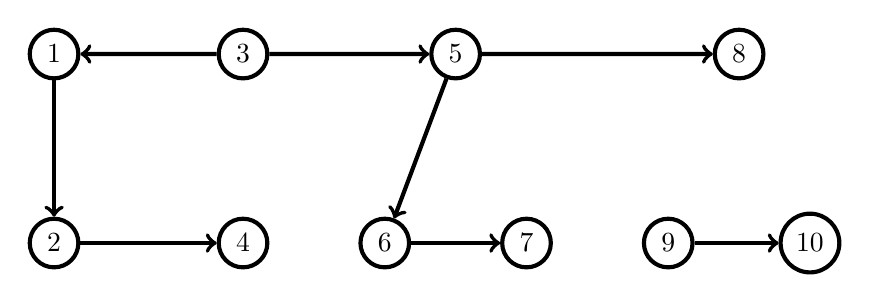
\begin{tikzpicture}[line width=1.5,scale=1.2]
 \node[circle,draw=black] (1) at (0,2) {$1$};
 \node[circle,draw=black] (2) at (0,0) {$2$};
 \node[circle,draw=black] (3) at (2,2) {$3$};
 \node[circle,draw=black] (4) at (2,0) {$4$};
 \node[circle,draw=black] (5) at (4.25,2) {$5$};
 \node[circle,draw=black] (6) at (3.5,0) {$6$};
 \node[circle,draw=black] (7) at (5,0) {$7$};
 \node[circle,draw=black] (8) at (7.25,2) {$8$};
 \node[circle,draw=black] (9) at (6.5,0) {$9$};
 \node[circle,draw=black] (10) at (8,0) {$10$};
		
 \draw[->] (1) edge (2);
 \draw[->] (2) edge (4);
 \draw[->] (3) edge (1) (3) edge (5);
 \draw[->] (5) edge (6) (5) edge (8); 
 \draw[->] (6) edge (7);
 \draw[->] (9) edge (10);
\end{tikzpicture}
\end{center} 
\end{bsp} 

\begin{bem}
		Wir bezeichnen die Tiefensuche kurz als $\cc{TS}$, die vollständige Tiefensuche als $\cc{VTS}$ und die Intialisierung der Tiefensuche als $\cc{TSI}$. 
\end{bem} 

\begin{lem} \label{ts:key:lemma} 
	Sei $D=(V,A)$ Digraph, sei $s \in V$ und man betrachte die Ausführung von $\cc{TS}(s)$ nach einer Initialisierung der Tiefensuche für $D$. Während der Ausführung ist  nach jeder Knotenfärbung  Folgendes erfüllt:
	\begin{enuma} 
		\item Die Menge der grauen Knoten bildet einen gerichteten Weg $(u_0,\ldots,u_m)$ in $D_\pi$, der im Knoten $u_0=s$ beginnt. 
		\item Der Kontrollfluss befindet sich im Aufruf von $\cc{TS}(u_m)$. 
		\item Für jedes $i=1,\ldots,m$ wurde $\cc{TS}(u_i)$  aus $\cc{TS}(u_{i-1})$ aufgerufen und die Aufrufe $\cc{TS}(u_1),\ldots,\cc{TS}(u_m)$ sind noch nicht zu Ende ausgeführt. 
	\end{enuma} 
	Darüber hinaus gilt: ein Knoten $v$ wird während Ausführung genau dann entdeckt, wenn in $D$ ein $(s,v)$-Pfad existiert. 
\end{lem} 
\begin{proof}
	Für Behauptungen (a)--(c) benutzen wir die Induktion über die Anzahl der Färbungen während der Ausführung von $\cc{TS}(s)$. Die erste Färbung ist die Färbung von $s$ mit Grau. In diesem Moment der Ausführung gilt die Behauptung für  den Weg der Länge $0$, der aus dem Knoten $s$ besteht. Angenommen, die Behauptungen gelten nach $k \in\N$ Färbungen. Man betrachten den Pfad $(u_0,\ldots,u_m)$, für den die Behauptungen gelten. 
	
	Wird während der Ausführung von $\cc{TS}(u_m)$, ein weißer Knoten $v$ entdeckt, so wird $\cc{TS}(v)$ aufgerufen, in der $v$ grau gefärbt wird, sodass nach $k+1$ Färbungen die Behauptung für den Pfad $(u_0,\ldots,u_m,v)$ erfüllt wird. 
	
	Sind während der Ausführung von $\cc{TS}(u_m)$ alle von $u_m$ ausgehende Kanten sondiert, so wird $u_m$ schwarz gefärbt, die Ausführung von $\cc{TS}(u_m)$ terminiert und der Kontrollfluss kehrt zum Aufruf $\cc{TS}(u_{m-1})$. In diesem Fall gelten die Behauptungen nach $k+1$ Färbungen für den Pfad $(u_0,\ldots,u_{m-1})$. 
	
	Nun zeigen wir die letzte Behauptung: wenn ein Knoten $v$ entdeckt wird, dann bilden laut der Behauptung (a) die Knoten, die im Moment der Entdeckung von $v$ grau sind, einen $(s,v)$-Pfad. Umgekehrt, sei $v \in V$ ein Knoten, für welchen ein $(s,v)$-Pfad $(v_0,\ldots,v_t)$ in $D$ existiert. Wir zeigen, dass der Knoten $v$ entdeckt. Angenommen, das wäre falsch. Wir zeigen durch Induktion über $i=1,\ldots,t$, dass der Knoten $v_i$ entdeckt wird. Der Knoten $v_0=s$ wird entdeckt. Sei also $1 \le i < t$ und wir nehmen an, dass $v_0,\ldots,v_{i-1}$ entdeckt werden. Da $v_{i-1}$ entdeckt wird, wird die Kanten $(v_{i-1},v_i)$ sondiert, sodass $v_i$ spätestens beim Sondieren der Kante $(v_{i-1},v_i)$ entdeckt wird. 
\end{proof} 

\begin{kor} \label{kor:weisse:pfade} 
	Sei $D=(V,A)$ Digraph und sei $u \in V$.
	Sind die Farbattribute der Knoten von $V$ auf weiß/grau/schwarz gesetzt, und ist $u$ ein weißer Knoten, für den man $\cc{TS}(u)$ startet, so wird ein weißer Knoten $v \in V$ während der Ausführung von $\cc{TS}(u)$ genau dann entdeckt, wenn vor der Ausführung von $\cc{TS}(u)$ ein $(u,v)$-Pfad aus weißen Knoten existiert. 
\end{kor} 
\begin{proof}
	Bei der Ausführung von $\cc{TS}(u)$, wird die TS für Knoten, die vor der Ausführung grau oder schwarz waren, nicht aufgerufen. Somit entspricht der Ausführung von $\cc{TS}(u)$ einer Ausführung auf dem Teilgraphen von $D$, der durch Knoten induziert ist, welche vor der Ausführung weiß waren. Die Behauptung folgt also aus der letzten Behauptung von Lemma~\ref{ts:key:lemma}. 
\end{proof} 

\begin{lem}
	Sei $D= (V,A)$ Digraph. 
	Nach der Initialisierung der Tiefensuche und während der Ausführung von der vollständige Tiefensuche der Graph $D_\pi$ stets ein gerichteter Wald. Die Wurzel der Bäume dieses Waldes sind genau die Knoten $u \in V$, für welche $\cc{TS}(u)$ direkt aus der vollständigen Tiefensuche aufgerufen wurde. 
\end{lem} 
\begin{proof} 
	Die Anzahl der Knoten, die während der Ausführung entdeckt werden nimmt während der Ausführung zu. Am Anfang der Ausführung wird der Knoten $s$ entdeckt und grau gefärbt. Die Behauptung gilt also am Anfang der Ausführung. Wir führen Induktion nach der Anzahl der Färbungen mit der Farben Grau. Am Anfang ist kein Knoten grau gefärbt und kein Vorgänger gesetzt, sodass $D_\pi$ ein Wald ohne Kanten ist. 
\end{proof} 

\begin{thm} \label{thm:ts:und:zyklen} 
	Sei $D=(V,A)$ Digraph, sei $s \in V$ und man betrachte die Ausführung von $\cc{TS}(s)$ nach einer Initialisierung der Tiefensuche für $D$. Der Digraph $D$ enthält genau dann einen von $s$ aus erreichbaren Zyklus, wenn während der Ausführung beim Sondieren einer der Kanten $(u,v)$ die Farbe von $v$ grau ist. 
\end{thm}
\begin{proof}	
	Sei während der Ausführung beim Sondieren eine Kante $(u,v)$ die Farbe von $v$ grau. Nach Lemma~\ref{ts:key:lemma} bildet die Menge der Knoten, die Grau gefärbt sind einen $(s,u)$-Weg $(u_0,\ldots,u_m)$ mit $u_0=s$ und $u=u_m$. Der Knoten $v$ ist also ein Knoten $u_j$ auf diesem Weg. Somit ist $(u_j,\ldots,u_m,u_j)$ ein Zyklus in $D$. 
	
	Umgekehrt sei $Z$ ein Zyklus, der von $s$ aus durch einen Pfad erreichbar ist. Wir zeigen, dass während der bei der Sondierung einer Kante der Endknoten der Kante grau ist. Sei $u$ der Knoten im Zyklus $Z$, der während der Ausführung unter allen Knoten von $Z$ als erster entdeckt wird. Nach der Färbung von $u$ mit Grau existiert nach Lemma~\ref{ts:key:lemma} ein $(s,u)$-Pfad $(u_0,\ldots,u_m)$ mit $s=u_0$ und $u_m=u$, der keinen anderen Knoten von $Z$ außer $u$ enthält. Wir schreiben $Z$ als $(v_0,\ldots,v_t,v_0)$ mit $v_0=u$.  
	
	Unmittelbar vor der Entdeckung ist $v_0,\ldots,v_t$ ein Pfad aus weißen Knoten. Nach Korollar~\ref{kor:weisse:pfade} wird während der Ausführung von $\cc{TS}(u)$ der Knoten $v_t$ entdeckt. Wir wenden das Lemma~\ref{ts:key:lemma} zum Teilgraphen an, der durch die Knoten induziert wird, die unmittelbar vor der Entdeckung von $u$ weiß sind. Da  $(v_0,\ldots,v_t)$ ein Pfad in diesem Teilgraphen ist, wird $v_t$ während der Ausführung von $\cc{TS}(u)$ entdeckt. Bei der Entdeckung von $v_t$ gibt es zwei Arten von grauen Knoten.  Die Knoten, welche vor dem Aufruf von $\cc{TS}(u)$ grau gefärbt wurden, sind $u_0,\ldots,u_m$. Die Knoten, die während der Ausführung von $\cc{TS}(u)$ und bis zum Aufruf von $\cc{TS}(v_t)$ grau gefärbt wurden, bilden einen $(u,v_t)$-Weg. 
	
	Es folgt:  nach der Entdeckung von $v_t$ hat der Weg aus grauen Knoten die Form $(u_0,\ldots,u_m, w_1,\ldots,w_\ell)$ mit $w_\ell =v_t$ hat. Beim sondieren der Kante $(v_t,u)$ ist also die Farbe von $u=u_m$ grau. 
\end{proof}

\begin{defn}
	Bzgl. einer vollständigen Tiefensuche auf $D=(V,A)$ mit Startknoten $s$ definieren die \textbf{Lebenszeitintervall} eines Knoten $v \in V$ als die Menge
	\[
			I_u:=\setcond{t \in \Z}{ \cc{Grau}[u] \le t \le \cc{Schwarz}[u]}. 
	\]
\end{defn} 

\begin{thm}[Klammerungstheorem]
\label{thm:klammerung}
Bei der vollständigen Tiefensuche auf einem Digraphen $D=(V,A)$ ist für jedes Paar von Knoten $u$ und $v$ genau eine der drei folgenden Bedingungen erfüllt:
\begin{enuma}

 \item $I_u \cap I_v = \emptyset$  und weder $u$ noch $v$ ist im Tiefensuchwald ein Nachfahre des anderen.

 \item $I_u \subseteq I_v$ und $u$ ist im Tiefensuchwald ein Nachfahre von $v$.

 \item $I_v \subseteq I_u$ und $v$ ist im Tiefensuchwald ein Nachfahre von $u$.

\end{enuma}
\end{thm}
\begin{proof}
	Die Aussage ist symmetrisch bzgl. $u$ und $v$. Wir  nehmen also ohne Beschränkung der Allgemeinheit an, dass während der Ausführung der vollständigen Tiefensuche der Knoten $u$ als erster entdeckt wurde. Ist die Tiefensuche für $v$ nach der Terminierung der Tiefensuche für $u$ aufgerufen worden, so gilt $I_u \cap I_v = \emptyset$. Ansonsten ist die Tiefensuche für $v$ vor der Terminierung der Tiefensuche für $u$ aufgerufen worden. Das bedeutet, dass der Knoten $v$ während der Ausführung von $u$ entdeckt worden ist. Der Aufruf von $TS(v)$ erfolgt also durch eine Folge der geschachtelten rekursiven Aufrufen 
	\[
		TS(u) \xrightarrow{} \cdots \xrightarrow{} TS(v) 
	\] 
	Somit terminiert $TS(v)$ vor $TS(u)$. Es gilt also $I_v \subseteq I_u$ ist $v$ ist Nachfahre von $u$. 
\end{proof}


\begin{bsp} 
	Die Relation der Lebenszeit Intervallen zu einander kann durch geklammerte Ausdrücke dargestellt werden. 
	Zur Illustration dieses Zusammenhangs sehen wir uns wieder die Tiefensuche aus Beispiel~\ref{bsp:tiefensuche} an.
	Die Daten der Zeitstempel sind in folgender Tabelle zusammengefasst:
	\begin{table}[H]
		\centering
		\begin{tabular}{|c|c|c|c|c|c|c|c|c|c|c|}
			\hline
			\textbf{Knoten $u$}        & \textbf{1} & \textbf{2} & \textbf{3} & \textbf{4} & \textbf{5} & \textbf{6} & \textbf{7} & \textbf{8} & \textbf{9} & \textbf{10} \\ \hline
			\textbf{$\cc{Grau}[u]$}    & 2          & 3          & 1          & 4          & 8          & 9          & 10         & 13         & 17         & 18          \\ \hline
			\textbf{$\cc{Schwarz}[u]$} & 7          & 6          & 16         & 5          & 15         & 12         & 11         & 14         & 20         & 19          \\ \hline
		\end{tabular}
	\end{table}
	Nach obiger Vorschrift können wir damit den zugehörigen Klammerausdruck
	\[
	(3\ (1\ (2\ (4\ 4)\ 2)\ 1)\ (5\ (6\ (7\ 7)\ 6)\ (8\ 8)\ 5)\ 3)\ (9\ (10\ 10)\ 9)
	\]
	ablesen.
	
	Eine andere Möglichkeit diese Klammerstruktur auszudrücken ist im folgenden Satz festgehalten:
\end{bsp} 


\begin{bem}
Als direkte Konsequenz des Klammerungstheorems erhalten wir eine Charakterisierung der Nachfahren im Tiefensuchwald eines gegebenen Knotens.
\end{bem} 

\begin{kor}
\label{cor:nachfahre-tiefenwald}
Der Knoten $v$ ist in einem Tiefensuchwald eines Digraphen genau dann ein echter Nachfahre eines Knotens $u$, wenn
\[
\cc{Grau}[u] < \cc{Grau}[v] < \cc{Schwarz}[v]  < \cc{Schwarz}[u].
\]
\end{kor}

\begin{bem} 
Eine alternative Charakterisierung der Nachfahreneigenschaft in Tiefensuchwäldern, die allerdings über die Farben der Knoten während der Suche geht, wird uns später bei den Anwendungen der Tiefensuche nützlich sein. 
\end{bem}


\begin{defn}
\label{def:kantenarten-tiefensuche}
Die Kanten $(u,v) \in A$ die bei einer Tiefensuche auf $D=(V,A)$ sondiert werden, werden in Abhängigkeit davon, welche Farbe $v$ beim Sondieren von $(u,v)$ hat und in welchem Zusammenhang $\cc{Grau}[u]$  und $\cc{Grau}[v]$ stehen, in die folgenden Arten unterteilt: 
\begin{center} 
\begin{tabular}{l|l}
	Art von $(u,v) \in A$ & Bedingung beim Sondieren 
	\\ \hline 
	\textbf{Baumkante} & $\cc{Farbe}[v]=\cc{weiss}$ 
\\	\textbf{Rückwärtskante} & $\cc{Farbe}[v] = \cc{grau}$
\\ \textbf{Vorwärtskante} & $\cc{Farbe}[v] = \cc{schwarz}$, $\cc{Grau}[u] < \cc{Grau}[v]$
\\ \textbf{Querkante} & $\cc{Farbe}[v] = \cc{schwarz}$, $\cc{Grau}[u] > \cc{Grau}[v]$
\end{tabular} 
\end{center} 
Baumkanten sind die Kanten des Tiefensuchwalds $D_\pi$. 
\end{defn}

\begin{bsp} Im Fall der Adjazensliste 
	\begin{align*}
		 1: & \ [2,4] 
		 \\ 2: & \  [3,4]
		 \\ 3: & \ [1]
		 \\  4: & \ [3]
	\end{align*}
 wird  während der Ausführung von $\cc{Tiefensuche}(1)$ die folgende Unterteilung der Kanten in die vier Arten festgelegt: 
	\begin{center} 
	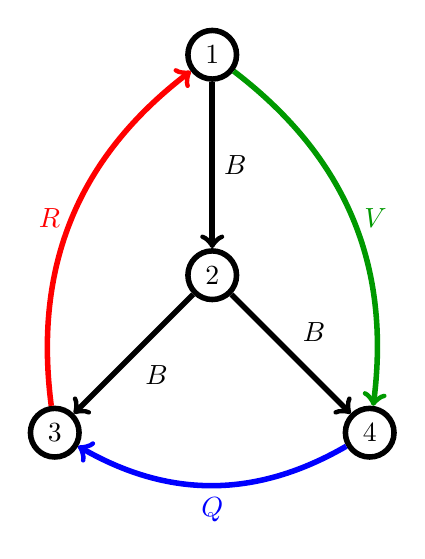
\begin{tikzpicture}[line width=2,scale=2]
		\node[circle,draw=black] (1) at (0,3.4) {$1$};
		\node[circle,draw=black] (2) at (0,2) {$2$};
		\node[circle,draw=black] (3) at (-1,1) {$3$};
		\node[circle,draw=black] (4) at (1,1) {$4$};
		\draw[->] (1) edge node[right]{$B$}(2) (2) edge node[below right]{$B$} (3) (2) edge node[above right]{$B$} (4);
		\draw[->,red] (3) edge[bend left] node[left]{$R$} (1);
		\draw[->,green!60!black]  (1) edge[bend left] node[right]{$V$} (4);
		\draw[->,blue] (4) edge[bend left] node[below]{$Q$} (3);
	\end{tikzpicture} 
	\end{center} 
\end{bsp} 

\begin{prop} 
	Wird die Unterteilung der Kanten in die vier Arten Baum-, Rückwärts- Vorwärts- und Querkante im Rahmen der vollständigen Tiefensuche durchgeführt, so ist jede Kante, welche zwei Bäume des Tiefensuchbaums verbindet eine Querkante. 
\end{prop} 


%\begin{remark}
%Durch die TS können die Kanten $(u,v)$ des Graphen in drei Arten klassifiziert werden: die Vorwärtskanten (beim sondieren von $(u,v)$ ist $v$ weiß), die Rückwärtskarten (beim sondieren der Kante ist $v$ grau) und die Querkanten (beim Sondieren der Kante ist $v$ schwarz). Die Menge aller  $\{u,v\}$ derart, dass $(u,v) \in E$ als ein Vorwärtskante klassifiziert wurde, ist Kantenmenge eines Baums. Die Knotenmenge dieses Baums ist die Menge aller entdeckten Knoten.
%\end{remark}

\begin{bsp} 
Wir schauen uns wiederum die Tiefensuche aus Beispiel~\ref{bsp:tiefensuche} an und, basierend auf den bereits erhobenen Daten, stellen wir die Klassifikation der Kanten des bearbeiteten Digraphen farbkodiert in folgender Abbildung dar.
Dabei sind Baumkanten schwarz, Rückwärtskanten rot, Vorwärtskanten blau und Querkanten grün markiert.

\begin{center} 
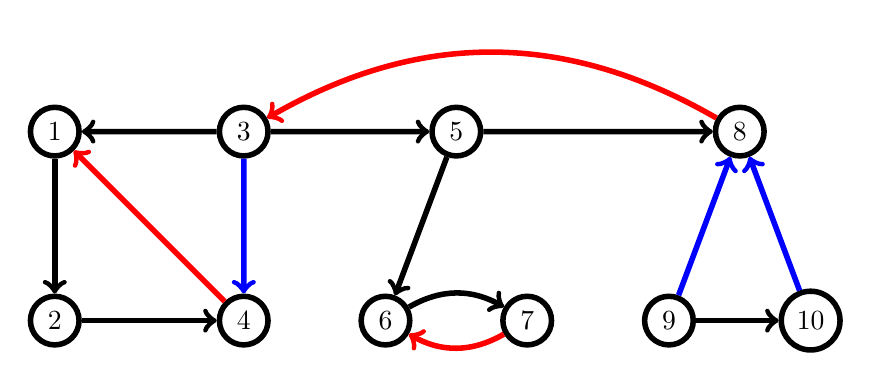
\begin{tikzpicture}[line width=2,scale=1.2]
 \node[circle,draw=black] (1) at (0,2) {$1$};
 \node[circle,draw=black] (2) at (0,0) {$2$};
 \node[circle,draw=black] (3) at (2,2) {$3$};
 \node[circle,draw=black] (4) at (2,0) {$4$};
 \node[circle,draw=black] (5) at (4.25,2) {$5$};
 \node[circle,draw=black] (6) at (3.5,0) {$6$};
 \node[circle,draw=black] (7) at (5,0) {$7$};
 \node[circle,draw=black] (8) at (7.25,2) {$8$};
 \node[circle,draw=black] (9) at (6.5,0) {$9$};
 \node[circle,draw=black] (10) at (8,0) {$10$};

% Baumkanten
 \draw[->] (1) edge (2);
 \draw[->] (2) edge (4);
 \draw[->] (3) edge (1) (3) edge (5);
 \draw[->] (5) edge (6) (5) edge (8); 
 \draw[->] (6) to[bend left] (7);
 \draw[->] (9) edge (10);

% Rückwärtskanten
 \draw[->,red] (4) edge (1);
 \draw[->,red] (7) to[bend left] (6);
 \draw[->,red] (8) to[bend right] (3);

% Vorwärtskanten
 \draw[->,blue] (3) edge (4);
 \draw[->,blue] (9) edge (8);
 \draw[->,blue] (10) edge (8); 
	
% Querkanten (keine vorhanden..)
	
\end{tikzpicture}
\end{center} 
\end{bsp} 


\begin{thm}
Bei einer Tiefensuche auf einem ungerichteten Graphen $G$ ist jede Kante entweder eine Baumkante oder eine Rückwärtskante.
\end{thm}

\begin{proof}
Sei $(u,v)$ eine beliebige Kante von~$G$ und seien die Knoten so bezeichnet, dass $\cc{Grau}[u] < \cc{Grau}[v]$ gilt.
Die Tiefensuche muss daher den Knoten~$v$ entdeckt und fertig abgearbeitet haben, bevor~$u$ fertig abgearbeitet ist.
In der Zwischenzeit ist der Knoten~$u$ stets grau.
Falls die Durchmusterung die Kante zuerst in der Richtung von~$u$ nach~$v$ sondiert, so ist~$v$ bis dahin unentdeckt (also weiß) gewesen, da die Kante sonst bereits in Gegenrichtung sondiert worden wäre.
Mit anderen Worten, die Kante $(u,v)$ ist eine Baumkante.

Falls nun die Durchmusterung die Kante zuerst in der Richtung von~$v$ nach~$u$ sondiert, so ist die Kante $(u,v)$ eine Rückwärtskante, da~$u$ zu dem Zeitpunkt der Sondierung noch grau ist.
\end{proof}


\begin{bem}
	Analog zur diskutierten Breitensuche kann man eine \emph{Tiefensuche} auch ohne Rekursion umsetzen.
	Dies hat praktische Vorteile, weil der Programmstack nicht  belastet wird.
	Dazu ersetzt man die Warteschlange $Q$ durch einen sogenannten \emph{Stack} ($=$ \emph{Stapel}). Für die Tiefensuche kann ein Stack auf der Basis von einem Array umgesetzt werden. 
	
	Hier eine ziemlich direkte Konvertierung der rekursiven Umsetzung. Wir gehen von einem zugrundeliegenden Stack $S$ aus. Als $\cc{Top}(S)$ bezeichnen wir das oberste Element des Stacks . Durch $\cc{Pop}(S)$ erfolgt die Entfernung und Rückgabe des obersten Elements. Durch $\cc{Push}(S,u)$ wird ein neues Element $u$ auf den Stack gelegt. Die Elemente $N[u]$ indexieren wir mit Zahlen $0$ bis $\deg(u)-1$, wobei hier $\deg(u)$ der Grad des Knotens $u$ ist. Wir führen ein Array $\cc{ind}$ ein, in dem durch $\cc{ind}[u]$ notiert wird, dass beim Sondieren der Nachbarn von $u \in V$  der Knoten $v=N[u][\cc{ind}[u]]$ als  nächster dran ist. Ist $\cc{ind}[u]= \deg(u)$, so hat man alle Nachbarn von $u$ sondiert. Wir setzen am Anfang $\cc{ind}[u]=0$ für alle $u \in V$, färben den Startknoten $s$ grau und legen $s$ auf $S$. Auf diese Weise lassen sich mit Hilfe von $S$ und $\cc{ind}$ die gerade laufenden rekursiven Aufrufe der Tiefensuche simulieren: 
	
	\begin{algorithm}[H]
		\caption{$\cc{Tiefensuche-mit-Stack}(s)$} 
		\begin{algorithmic}[1]
			\STATE Stack $S$ für höchstens $|V|$ Elemente anlegen
			\STATE $\cc{Farbe}[s] = \cc{grau}$ 
			\STATE $\cc{push}(S,s)$
			\STATE Liste $\cc{Ind}$  mit $\cc{Ind}[u]=0$ für alle $u \in V$ anlegen
			\WHILE{$S$ nicht leer }
			\STATE $u:= \cc{top}(S)$ \quad \COMMENT{Suche für $u$ läuft weiter}
			\IF{$\cc{ind}[u] = \deg(u)$} 
			\STATE $\cc{pop}(S)$   \quad \COMMENT{Suche für $u$ wird beendet}
			\STATE $\cc{Farbe}[u] := \cc{schwarz}$
			\ELSE
			\STATE $v=N[u][\cc{ind}[u]]$ \quad \COMMENT{Sondierung der Nachbarn von $u$ wird fortgesetzt} 
			\STATE $\cc{ind}[u]:=\cc{ind}[u]+1$				
			\IF{$\cc{Farbe}[v] = \cc{weiss}$}
			\STATE $\cc{Farbe}[v] = \cc{grau}$ \quad \COMMENT{Neuer Knoten ist entdeckt}
			\STATE $\cc{push}(S,v)$ \quad \COMMENT{Suche für $v$ wird gestartet}
			\ENDIF 
			\ENDIF 
			\ENDWHILE  
		\end{algorithmic}
	\end{algorithm}
	
	Die weiteren Daten, die man im Rahmen der rekursiven Tiefensuche berechnen kann, kann man auch in der obigen iterativen Version an den entsprechenden Stellen berechnen. 
\end{bem}

\begin{bem}\ Umsetzung: 
\lstinputlisting{Code/dfs.sage}
\end{bem} 


\subsection{Anwendung I -- Topologisches Sortieren}

\begin{defn} 
Sei $D=(V,A)$ ein Digraph mit $n$ Knoten.
Eine \emph{topologische Sortierung} von $D$ ist eine Anordnung $v_1,\ldots,v_n$ seiner Knoten, so dass $i < j$ gilt, falls $(v_i,v_j) \in A$ eine Kante in~$D$ ist.
Das heißt, der Startknoten einer jeden Kante kommt in der Anordnung vor dem Endknoten.
\end{defn} 

\begin{bem}
Man kann die topologische Sortierung auch als horizontale Anordnung der Knoten von~$D$ auffassen, so dass jede Kante von links nach rechts zeigt.

Diese Veranschaulichung zeigt, dass es nicht möglich ist, einen Digraphen topologisch zu sortieren, wenn er einen Zyklus enthält.
Im Folgenden werden wir sehen, wie man mit einer Tiefensuche jeden \emph{azyklischen} Digraphen topologisch sortieren kann.
Als Konsequenz ergibt sich:
\end{bem} 

\begin{prop}
Ein Digraph besitzt genau dann eine topologische Sortierung, wenn er azyklisch ist.
\end{prop}

\begin{bem}
	Eine Anwendung des topologischen Sortierens ist \textbf{makefile}. Die Kanten des Diagraphen sind durch  die Paare target-prerequisite gegeben. Die targets sollen in einer topologisch sortierten Reihenfolge abgearbeitet werden. 
	
	Eine andere Anwendung ist das Sequenzieren von Aufträgen (engl.~\emph{scheduling}).
\end{bem}


\begin{thm}
	Nach der Ausführung der vollständigen Tiefensuche auf einem azyklischen Digraphen $D=(V,A)$ ist die Anordnung der Knoten $u \in V$ in der absteigenden Reihenfolge nach $\cc{Schwarz}[u]$ eine topologische Sortierung. Diese Anordnung kann während der Tiefensuche in der Zeit $\Theta(|V|+|A|)$ berechnet werden. 
\end{thm}

\begin{proof}
	Wir betrachten eine Kante $(u,v)$. Ist $v$ vor $u$ entdeckt worden, so wird während der Ausführung von $TS(u)$ der Knoten $u$ nicht entdeckt, denn sonst gäbe es einen $(v,u)$-Pfad und somit auch einen Zyklus in $D$. Das bedeutet, dass in diesem Fall $TS(v)$ vor $TS(u)$ terminiert. Es gilt also $\cc{Schwarz}[v] \le \cc{Schwarz}[u]$. 
	
	Wird $u$ vor $v$ entdeckt, so wird $v$ während der Ausführung von $TS(u)$ spätestens beim Sondieren von $(u,v)$ entdeckt. In diesem Fall terminiert $TS(v)$ ebenfalls vor $TS(u)$. Somit gilt auch in diesem Fall $\cc{Schwarz}[v] \le \cc{Schwarz}[u]$.
\end{proof}




\subsection{Anwendung II -- Starke Zusammenhangskomponenten}

\begin{defn}
	Knoten $u,v \in V$ eines Digraphen $D=(V,A)$ heißen \textbf{gegenseitig erreichbar} wenn ein $(u,v)$-Pfad sowie ein $(v,u)$-Pfad existiert. Gegenseitige Erreichbarkeit ist eine Äquivalenzrelation auf $V$. Die Äquivalenzklassen bzgl. dieser Relation nennt man \textbf{starke Zusammenhangskomponenten} (SZK) von $D$. 
\end{defn} 

\begin{bsp}
	In diesem Beispiel sind die starkten Zusammenhangskomponenten mit mehr als einem Knoten farbich hinterlegt: 
\begin{center}
	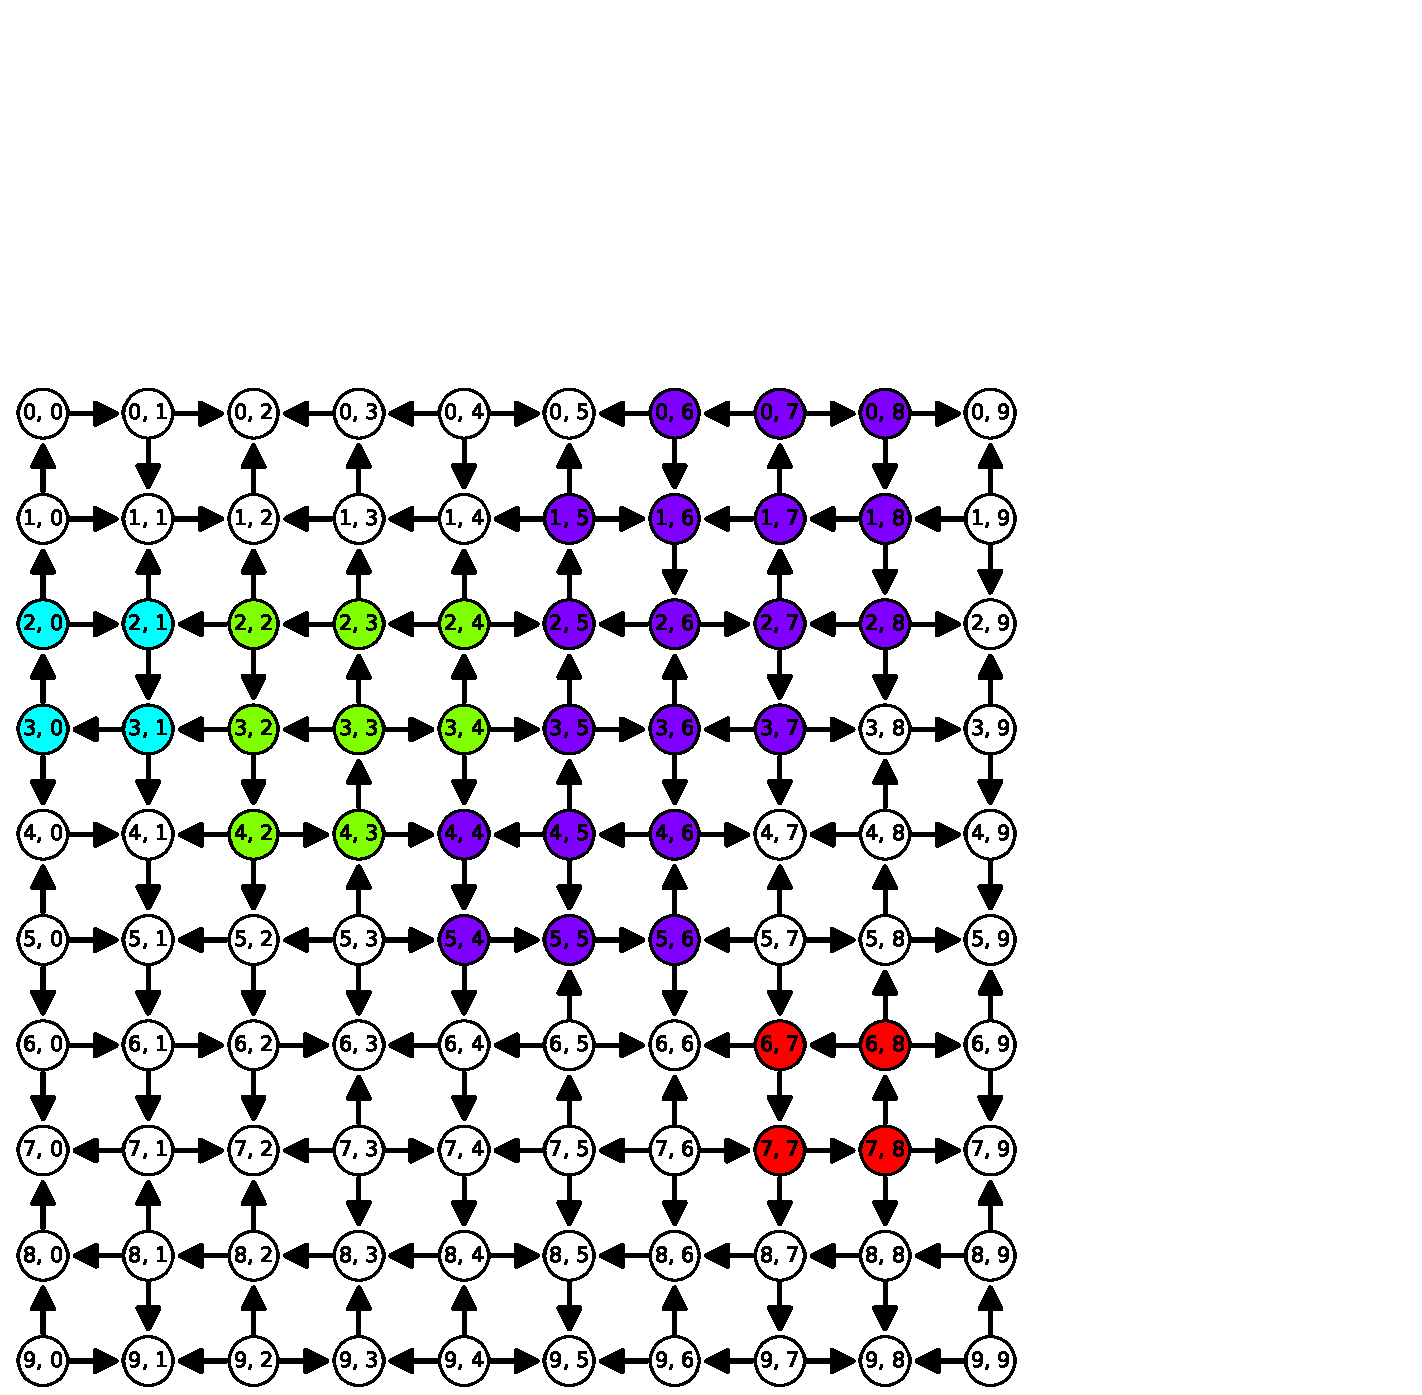
\includegraphics[width=0.5\textwidth]{Code/strongly_connected_comp.pdf}
\end{center} 
\end{bsp}

\begin{thm}
	\label{thm:starke-zshgk-laufzeit}
	Ist ein Digraph $D=(V,A)$ als Adjazenzliste gegeben, so hat der Algorithmus aus \ref{szk:algo} die Laufzeit $\Theta(|V|+|A|)$.
\end{thm}
\begin{proof}
	Die Berechnung von $D^\top$ sowie die beiden vollständigen Tiefensuchen sind benötigen jeweils  $\Theta(|V|+|A|)$ Elementaroperationen. 
\end{proof}

\begin{defn}
	Der \textbf{Komponentengraphen} $D^K=(V^K,A^K)$ eines Digraphen $D=(V,A)$
	ist ein Digraph, beim dem die Menge $V^K$ die Menge von SZK von $D$ ist und die Menge $A^K$ der Kanten die Menge aller paare $(U,W)$ mit $U,W \in V^K$ mit der Eigenschaft, dass  $(u,w) \in A$  für ein $u \in U$ und $w \in W$  erfüllt ist. 
\end{defn}

\begin{prop}
	Der Komponentengraph eines jeden Digraphen ist azyklisch. 
\end{prop}


\begin{bsp}
	\label{bsp:starke-zusammenhangskomponenten}
	Die starken Zusammenhangskomponenten des Digraphen aus Beispiel~\ref{bsp:tiefensuche} bestehen aus den Knoten gleicher Farbe in folgender Abbildung:
	
	\hfill
	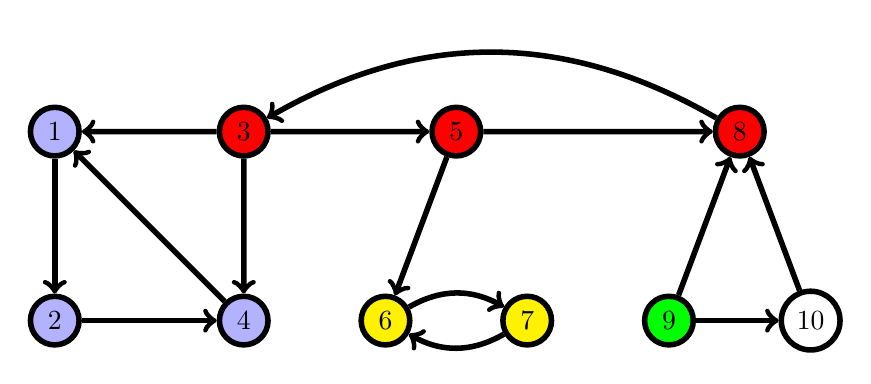
\begin{tikzpicture}[line width=2,scale=1.2]
		\node[fill=blue!30!white,circle,draw] (1) at (0,2) {$1$};
		\node[fill=blue!30!white,circle,draw] (2) at (0,0) {$2$};
		\node[fill=red,circle,draw] (3) at (2,2) {$3$};
		\node[fill=blue!30!white,circle,draw] (4) at (2,0) {$4$};
		\node[fill=red,circle,draw] (5) at (4.25,2) {$5$};
		\node[fill=yellow,circle,draw] (6) at (3.5,0) {$6$};
		\node[fill=yellow,circle,draw] (7) at (5,0) {$7$};
		\node[fill=red,circle,draw] (8) at (7.25,2) {$8$};
		\node[fill=green,circle,draw] (9) at (6.5,0) {$9$};
		\node[circle,draw=black] (10) at (8,0) {$10$};
		
		\draw[->] (1) edge (2);
		\draw[->] (2) edge (4);
		\draw[->] (3) edge (1) (3) edge (4) (3) edge (5);
		\draw[->] (4) edge (1);
		\draw[->] (5) edge (6) (5) edge (8); 
		\draw[->] (6) to[bend left] (7);
		\draw[->] (7) to[bend left] (6);
		\draw[->] (8) to[bend right] (3);
		\draw[->] (9) edge (8) (9) edge (10);
		\draw[->] (10) edge (8); 
	\end{tikzpicture}
	\hfill\,
\end{bsp}

Der Komponentengraph dieses  Digraphen ist: 
\begin{center} 
	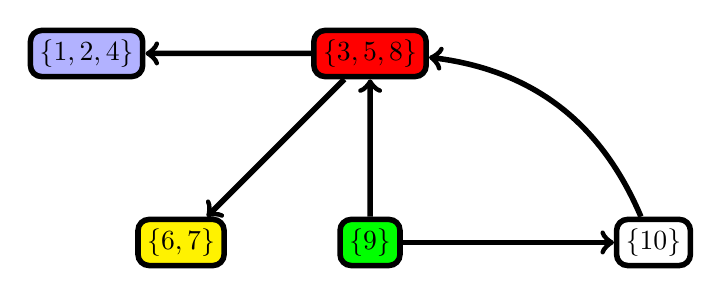
\begin{tikzpicture}[line width=2,scale=1.2]
		\node[fill=blue!30!white,rounded corners,draw] (1) at (3,2) {$\{1,2,4\}$};
		% \node[fill=blue,rounded corners,draw] (2) at (0,0) {$2$};
		% \node[fill=red,rounded corners,draw] (3) at (2,2) {$3$};
		% \node[fill=blue,rounded corners,draw] (4) at (2,0) {$4$};
		\node[fill=red,rounded corners,draw] (5) at (6,2) {$\{3,5,8\}$};
		\node[fill=yellow,rounded corners,draw] (6) at (4,0) {$\{6,7\}$};
		% \node[fill=yellow,rounded corners,draw] (7) at (5,0) {$7$};
		% \node[fill=red,rounded corners,draw] (8) at (7.25,2) {$8$};
		\node[fill=green,rounded corners,draw] (9) at (6,0) {$\{9\}$};
		\node[rounded corners,draw=black] (10) at (9,0) {$\{10\}$};
		
		\draw[->] (5) edge (6) (5) edge (1); 
		\draw[->] (9) edge (5) (9) edge (10);
		\draw[->] (10) to[bend right] (5); 
	\end{tikzpicture}
\end{center}


\begin{defn}
	Für einen Digraphen $D = (V,A)$ führen wir den sogenannten
 \emph{transponierten Graphen} $D^\top = (V,A^\top)$ mit $A^\top = \{(u,v) \in V \times V : (v,u) \in A\}$ ein. 
Wir erhalten also $D^\top$ aus $D$, indem wir die Orientierung aller Kanten von $D$ umdrehen.
\end{defn} 


\begin{prop}
\label{beob:d-vs-dt}
Der zu einem Digraphen $D=(V,A)$ transponierte Graph $D^\top$ hat dieselben starken Zusammenhangskomponenten wie~$D$.
\end{prop}

\begin{bem}  \label{szk:algo}
	Sei $D = (V,A)$ Digraph. Zur Berechnung der SZK von $D$ kann der folgende Algorithmus benutzt werden, den wir als $\cc{SZK}(D)$ bezeichnen: 
\begin{itemize}
	\item \textbf{Phase~1: Anordnung.} Ordne mit Hilfe der vollständigen Tiefesuche auf $D$ die Knotenmenge $V$ in absteigender Reihenfolge $u_1,\ldots,u_n$ der Abarbeitungszeit ($n:=|V|$). Es reicht dafür beim Abarbeiten eines Knoten, den Knoten zu einer Liste mit $n$ Elementen hinzuzufügen (und die Liste vom Ende beginnend zu füllen). 
	\item \textbf{Phase~2: Berechnung der Komponenten.} Für eine vollständige Tiefensuche auf $D^
\top$ durch, bei der  über die Knoten $u \in V$ in der oben bestimmten Reihenfolge $u_1,\ldots,u_n$ iteriert wird. Dabei entdeckt jeder Aufruf der Tiefensuche aus der vollständigen Tiefensuche die Knoten einer starken Zusammenhangskomponente.
\end{itemize} 

Wie man Phase~2 genau umsetzt hängt unter anderem davon ab, in welchem Format man die SZK speichern möchte. 
\end{bem} 

\begin{bem} Umsetzung: 
\lstinputlisting{Code/szk.sage}
\end{bem} 


\begin{thm}
$\cc{SZK}(D)$ bestimmt die starken Zusammenhangskomponenten eines Digraphen~$D=(V,A)$ korrekt.
\end{thm}


\begin{bem}
	Die Präsentation der Tiefensuche basiert auf  \cite{CLRS17}.
\end{bem} 